\subsection{ClientControl}
ClientControl er en tråd, som står for at læse fra- og skrive til klienters socket forbindelse.


\begin{figure}[H]
    \centering
    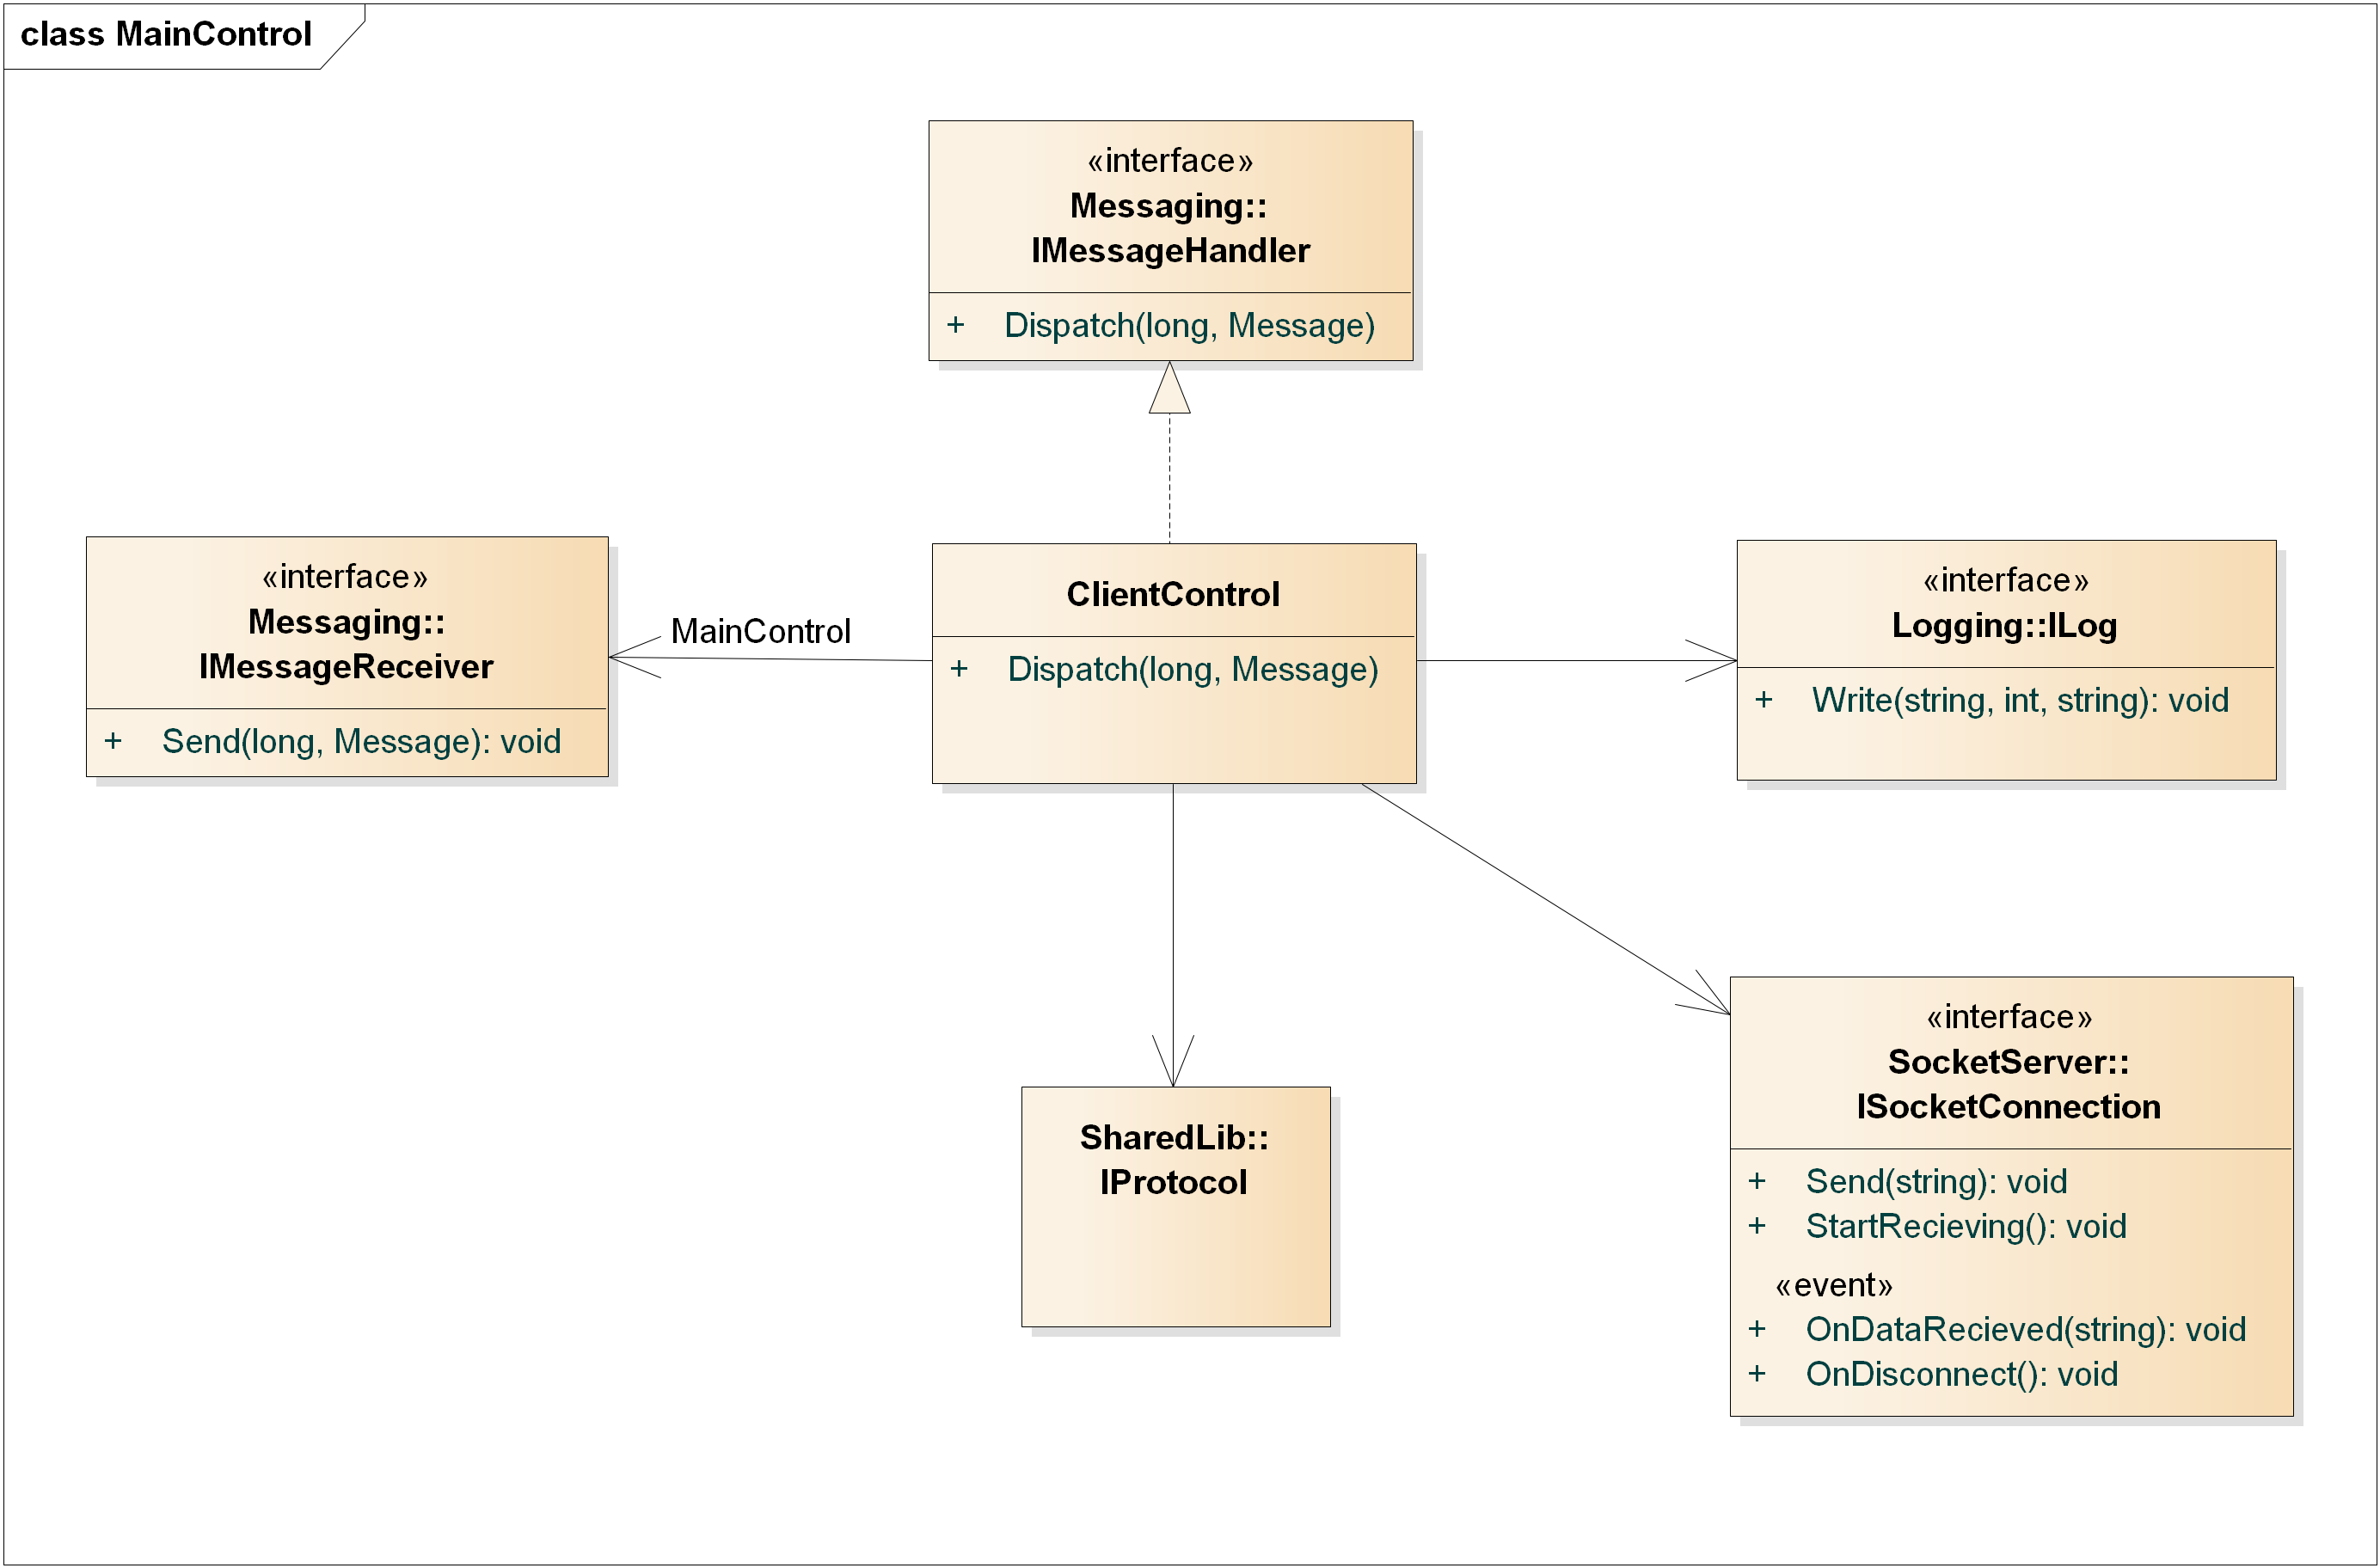
\includegraphics[width=1\textwidth]{Systemdesign/CentralServer/Images/ClientControl.png}
    \caption{UML-diagram for ClientControl}
    \label{fig:CSClientControl}
\end{figure}


\textbf{Events}\\
ClientControl kan modtage følgende events:\\

\textbf{E\_WELCOME}:
Når en klient forbinder sendes et E\_REGISTER\_CLIENT event til MainControl. Herefter sendes en E\_WELCOME til klienten (ClientControl) for at fortælle, at klienten er registreret, og at der kan begyndes at modtage data fra klienten.\\

\textbf{E\_SEND\_COMMAND}:
Sendes fra MainControl, når der skal sendes en kommando til klienten.\\